\documentclass{article}
\usepackage[T1]{fontenc}
\usepackage{lmodern}
\usepackage{graphicx}
\usepackage{amsmath,amssymb}
\usepackage[a4paper,margin=2cm]{geometry}
\usepackage[absolute,overlay]{textpos}
\setlength{\TPHorizModule}{1mm}
\setlength{\TPVertModule}{1mm}
\usepackage[indonesian]{babel}
\usepackage{hyperref}
\setlength{\emergencystretch}{2em}
% unit: Halaman 111

\begin{document}

% === Halaman 111 (llm) ===

\vspace{162.16mm}

\begin{itemize}
    \item Enigma menggunakan sistem rotor (roda berputar) untuk membentuk huruf cipherteks yang berubah-ubah.
    \item Setiap rotor melakukan substitusi abjad-tunggal (monoalphabetic cipher).
    \item Hasil substitusi oleh suatu rotor menjadi huruf input untuk operasi substitusi rotor selanjutnya.
    \item Hasil substitusi oleh rotor terakhir menjadi huruf cipherteks.
    \item Setiap kali sebuah huruf dienkripsi oleh sebuah rotor, rotor berputar satu huruf untuk membentuk huruf cipherteks baru bagi huruf plainteks berikutnya.
\end{itemize}

\vspace{20mm}

\begin{itemize}
    \item Setelah berputar 26 huruf rotor kembali pada posisi semula. Jadi, diperoleh cipher abjad-majemuk dengan periode 26.
\end{itemize}

% deskripsi: Foto detail mesin Enigma yang memperlihatkan rotor dan papan keyboard huruf.
% bbox normalisasi: [0.5170, 0.1410, 0.9680, 0.6870]
\begin{textblock*}{94.71mm}(108.57mm,41.88mm)
\noindent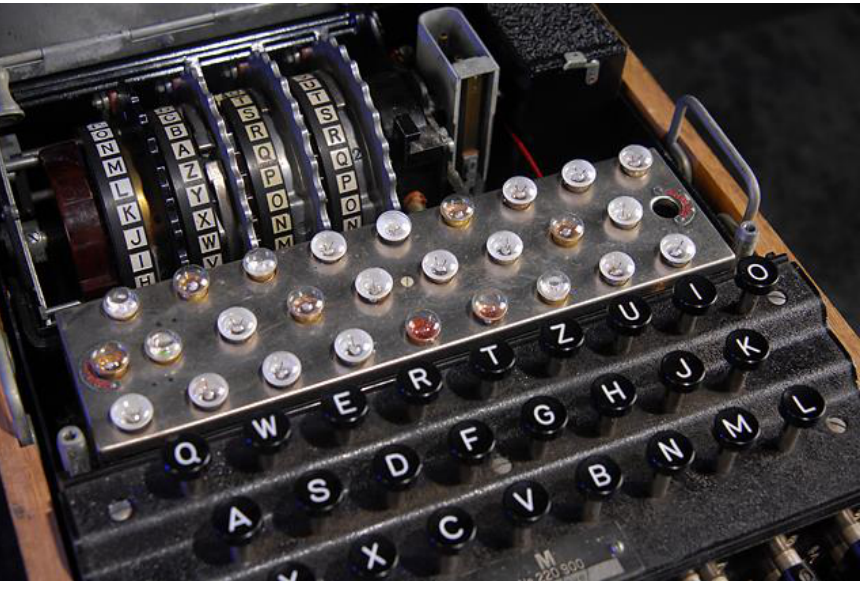
\includegraphics[width=94.71mm,height=162.16mm]{../../images/llm/page_111_img_01.png}%
\end{textblock*}

\end{document}
